\section*{Аннотация}
\indent В работе мы исследовали явления дифракции Френеля на щели, дифракции Фраунгофера на щели и на двух щелях, изучили влияние дифракции на разрешающую способность оптических инструментов.
\section*{Теоретические сведения}
\subsection*{\textit{Дифракция Френеля на щели}}

Для расчёта светового поля воспользуемся методом векторных диаграмм. Разбив щель на узкие полоски \( d\xi \), параллельные краям щели, изобразим колебание, созданное полоской в точке наблюдения \( P \). Разность фаз колебаний от полосок на расстояниях $\xi$ и $\xi + d\xi$
зависит от $\varepsilon$:

$$ d\varphi = \frac{k}{z}\xi d\xi$$

\begin{wrapfigure}[14]{r}{0.38\linewidth}
    \centering
    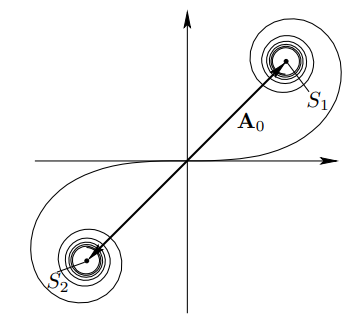
\includegraphics[width=6cm]{images/karnu.png}
    \caption{Спираль Корню}\label{fig:cornu}
\end{wrapfigure}

Поэтому угол между двумя соседними векторами на диаграмме не сохраняется неизменным.
По мере удаления от центра угол начинает быстро нарастать - цепочка векторов быстро скручивается.
Суммарный вклад всей полосы изображается вектором A1, проведённым из начала первого вектора в конец последнего.
Продолжая дальше построение векторной диаграммы, придём к спирали Корню, изображённой на рис.~\ref{fig:cornu}. Спираль, быстро скручиваясь, приближается к точке \(S_1\), называемой фокусом спирали. Каждый последующий полувиток спирали изображает вклад в суммарное колебание последовательно расположенных зон Шустера, причём \(m\)-я зона Шустера - это полоса, внешний край которой отстоит от точки наблюдения на расстояние \(z + m\sqrt{2}\) и на расстояние

\begin{equation}
\xi_m = \sqrt{m\lambda z}, \quad m = 1, 2, 3, \ldots, \label{eq:xi_m}
\end{equation}
\begin{figure}[h!]
    \centering
    \begin{subfigure}{0.48\linewidth}
        \centering
        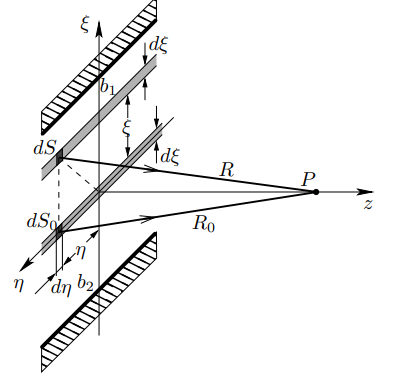
\includegraphics[width=7cm]{images/A_theory.png}
        \caption{Дифракция Френеля на щели}
    \end{subfigure}
    \hfill
    \begin{subfigure}{0.5\linewidth}
        \centering
        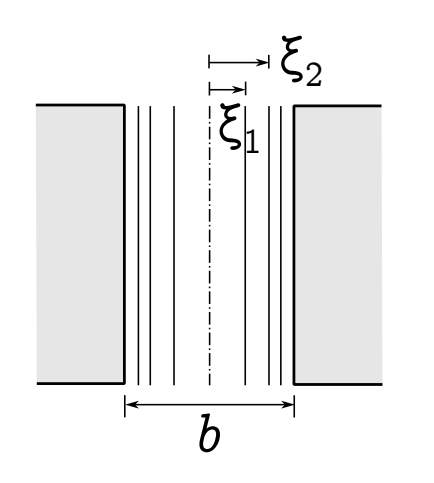
\includegraphics[width=6cm]{images/shuster_zones.png}
        \caption{Зоны Шустера в плоскости щели}
    \end{subfigure}
\end{figure}

\indent Дифракция Френеля наблюдается, когда количество окткрытых зон Френеля (Шустера) порядка единицы:
\begin{equation}
    m = \frac{b^2}{\lambda z} \sim 1
\end{equation}

\subsection*{\textit{Дифракция Фраунгофера на щели}}
Для нахождения картины Фраунгоферовой дифракции, необходимо найти преобразование Фурье граниченого поля $f_0(x)$ в плоскости $z = 0$ (аналогичнo нахождению спектра прямоугольного импульса - роль длительности импульса здесь
играет ширина щели b, а роль частоты - пространственная частота $u = k \sin\theta$). Получаем:

\begin{equation}
    g(\theta) = g(\theta) \propto \int_{-b/2}^{+b/2} e^{ikx \sin \theta} \, dx \propto \frac{\sin \left( \frac{kb}{2} \sin \theta \right)}{\frac{kb}{2} \sin \theta} \label{eq:fraunogofer}
\end{equation}

\begin{figure}[h!]
    \centering
    \begin{subfigure}{0.38\linewidth}
        \centering
        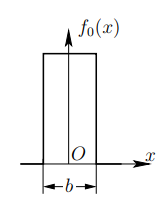
\includegraphics[width=4cm]{images/fraungofer_1.png}
        \caption{Поле на щели}
    \end{subfigure}
    \hfill
    \begin{subfigure}{0.6\linewidth}
        \centering
        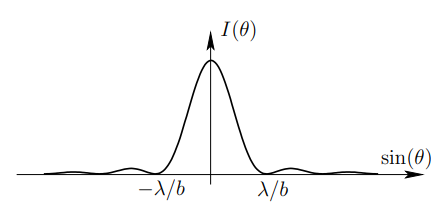
\includegraphics[width=9cm]{images/fraungofer_2.png}
        \caption{Угловое распределение интенсивности при дифракции Фраунгофера на щели}
    \end{subfigure}
\end{figure}

\indent Из формулы \ref{eq:fraunogofer} следует, что подавляющая величина потока энергии сосредоточена  в угловом конусе:
\begin{equation}
    |\sin\theta| \le \frac{\lambda}{b}
\end{equation}
С уменьшением ширины щели уширяется пространственный спектр - спектр плоских волн, бегущих от щели.

\subsection*{\textit{Дифракция Фраунгофера на двух щелях}}

\begin{wrapfigure}[14]{r}{0.36\linewidth}
    \centering
    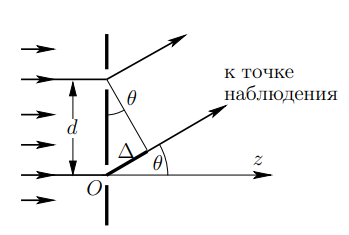
\includegraphics[width=6cm]{images/fraungofer_theory.png}
    \caption{К вычислению поля для дифракции Фраунгофера на двух щелях}
\end{wrapfigure}

Соответствующая фаза колебания отличается на величину:
\begin{equation}
    \alpha = -k\Delta = -k d\sin\theta
\end{equation}
Поэтому колебательный процесс, созданный второй щелью в точке наблюдения, описывается функцией $g(\theta)e^{i\alpha}$. Волны, посылаемые в точку наблюдения двумя щелями, интерферируют. Амплитуда суммарного колебательного процесса в точке наблюдения есть $g(\theta) + g(\theta)e^{i\alpha}$.
Картина интенсивности изображена ниже \ref{fig:intensity_fraungofer}:
\begin{equation}
    I(\theta) = |g(\theta)|^2 [1 + \cos(kd\sin\theta)]^2
\end{equation}
\begin{figure}[h!]
    \centering
    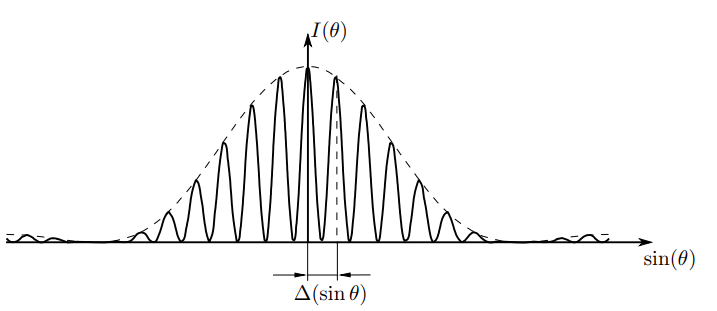
\includegraphics[width=14cm]{images/intensity_fraungofer.png}
    \caption{Зависимость интенсивности от угла для дифракции Фраунгофера на двух щелях}\label{fig:intensity_fraungofer}
\end{figure}





\section*{Экспериментальная установка}
\textit{\textbf{Оборудование:} оптическая скамья, ртутная лампа, светофильтр, щели с регулируемой шириной, рамка с вертикальной нитью, экран с двойной щелью, микроскоп на поперечных салазках с микрометрическим винтом, зрительная труба.}

\subsection*{А) Дифракция Френеля на щели}

\begin{figure}[h!]
\centering
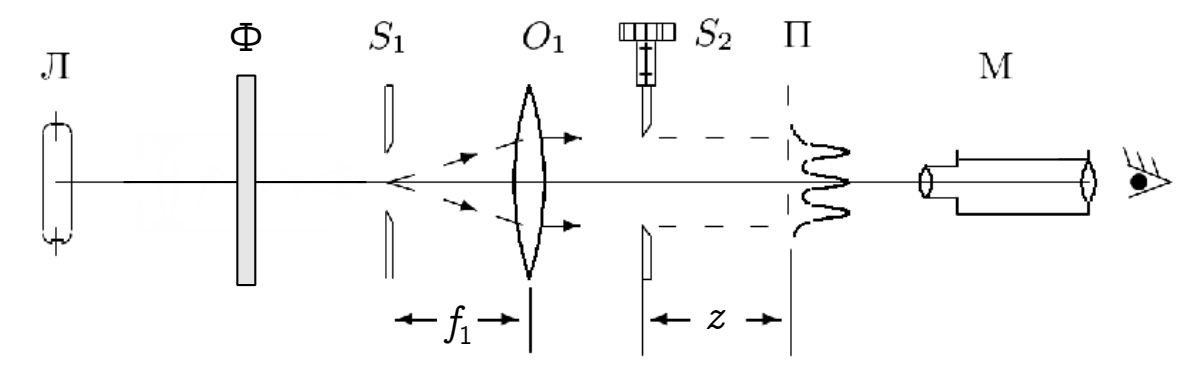
\includegraphics[width=12cm]{images/setup.png}
\caption{Экспериментальная установка для наблюдения дифракции Френеля}\label{fig:setup}
\end{figure}

\indent
Свет от ртутной ртутной ламы Л, пропущенный через оранжевый светофильтр Ф со средней
длиной волны $\lambda$ = 578 нм, падает на входную щель $S_1$. Щель $S_1$ находится в фокусе
коллиматора — собирающей линзы $O_1$. Коллиматор создаёт параллельный пучок монохроматического света, освещающий щель $S_2$, на которой и происходит дифракция. Дифракционная картина рассматривается с пoмощью микроскопа М, сфокусированного на некоторую плоскость наблюдения П.

\indent
Нашли резкое изображение щели (без дифракционных полос). Начальное положение микроскопа, имзеренное по шкале продольное линейки: $\mathbf{x_0 = 58.4}$ \textbf{cм}.\\\indent
Постепенно отодвигая микроскоп от щели S2, замерили по шкале положение микроскопа, при котором на фоне щели видно n  тёмных
полос. Результаты измерений приведены в
\begin{table}[h]
    \centering
    \begin{tabular}{|c|c|c|c|}
        \hline
        \( x_n \), мм & \( n \) & \( z_n\), мм & \( \xi_n \), мкм \\\hline
        574    & 6    & 10    & $181 \pm 11$   \\ \hline
        573    & 4    & 11    & $155 \pm 9 $   \\ \hline
        570    & 3    & 14    & $151 \pm 9 $   \\ \hline
        567    & 2    & 17    & $136 \pm 7 $   \\ \hline
        558    & 1    & 26    & $119 \pm 6 $   \\ \hline
    \end{tabular}
    \caption{Зависимость координат полос от числа видных темных полос} \label{table:measurements_A}
\end{table}

\text{где } $z_n = x_0 - x_n$\text{ - расстояние от щели до плоскости наблюдения; }$\sigma_{x_n} = 1$\text{ мм; } $\sigma_{a_n} = 1 $\text{ мм.} График изображен на рисунке \ref{fig:plot_A}.
\begin{figure}[!ht]
    \centering
    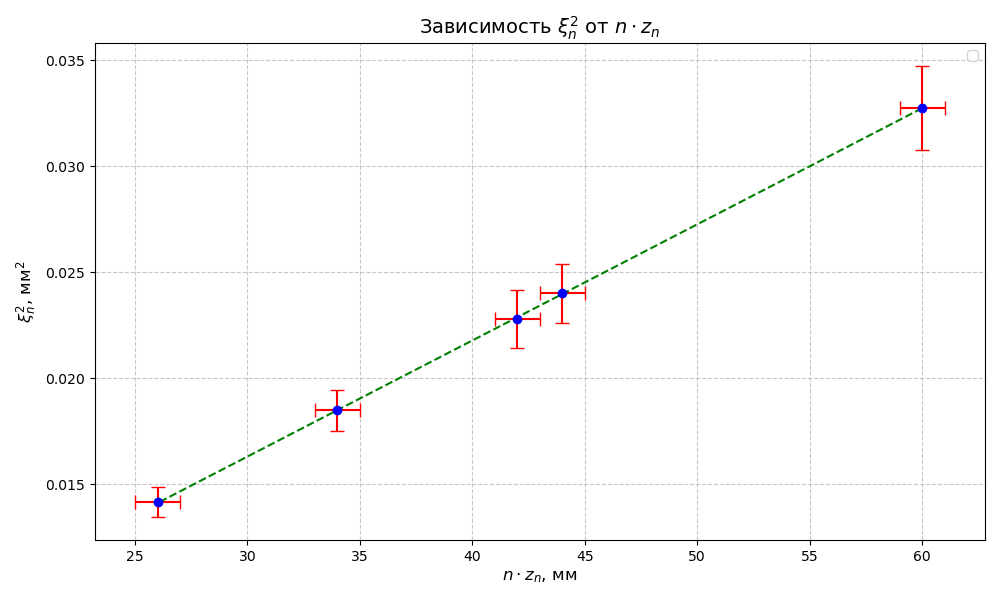
\includegraphics[width=18cm]{images/plot_A.png}
    \caption{К определению ширины щели b в случае диффракции Френеля на щели} \label{fig:plot_A}
\end{figure}
\noindent
Коэффициент наклона графика $k = \lambda_{g} = 547$ нм, что совпадает с табличным значением $\lambda_{g} = 546$ нм.
\\ Ширина щели получается $\mathbf{b = 0.155 \pm 0.025}$ \textbf{мм}. Ширина щели измеренная микрометрическим винтом: $\mathbf{b = 0.16 \pm 0.02}$ \textbf{мм}.

\subsection*{Б) Дифракция Фраунгофера на щели}
\begin{figure}[!ht]
    \centering
    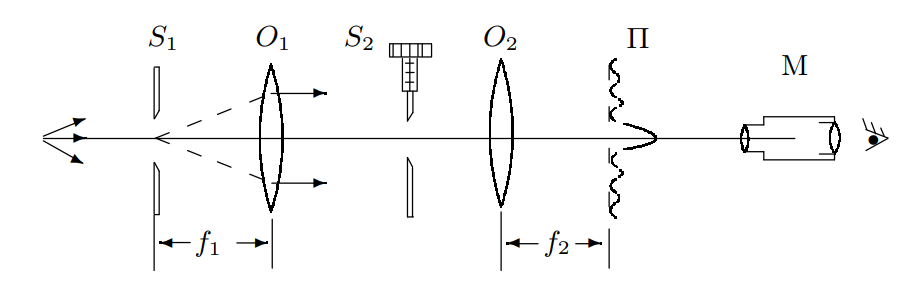
\includegraphics[width=12cm]{images/setup_2.png}
    \caption{Схема установки для наблюдения дифракции Фраунгофера на щели}
\end{figure}
Дифракцию Френеля и Фраунгофера можно наблюдать на одной и той же установке (\ref{fig:setup}). Однако при обычных размерах установки дифракция Фраунгофера возникает только при очень узких щелях. Поэтому к прошлой установке добавляется объектив O2.\\\indent
Дифракционная картина наблюдается здесь в фокальной плоскости объектива O2. Каждому значению угла $\theta$ соответствует в этой плоскости точка, отстоящая от оптической оси на расстоянии:
\begin{equation}
    x = f_2 \tg\theta\approx f_2\theta
\end{equation}
\indent Поскольку объектив не вносит дополнительной разности хода
между интерферирующими лучами (таутохронизм), в его фокальной
плоскости наблюдается неискажённая дифракционная картина Фраунгофера. Эта картина соответствует бесконечно удалённой плоскости
наблюдения.
При малых углах $\theta$ положение тёмных полос определяется соотношением
\begin{equation}
    \theta_m = \frac{m\lambda}{b}
\end{equation}
\indent
Расстояние $x_m$ от тёмной полосы до оптической оси объектива O2 пропорционально фокусному расстоянию f2:
\begin{equation}
    x_m = m\frac{\lambda}{b}f_2 \label{eq:fraunogofer1_1}
\end{equation}

\indent
Ширина щели S2: $\mathbf{b = 0.28\pm 0.01}$ \textbf{мм}. Фокусное расстояние линзы O2: $\mathbf{f_2 = 11}$ \textbf{см}.
Измерили с помощью винта поперечного перемещения микроскопа координаты $X_m$ нескольких дифракционных минимумов. Результаты приведены в таблице \ref{table:measurements_2}.

По наклону прямой из графика \ref{fig:plot_B}, согласно формуле \ref{eq:fraunogofer1_1}, определили ширину щели S2:
$$
\mathbf{b = \frac{f_2\lambda}{k} = 0.24 \pm 0.05}\textbf{ мм}
$$
\begin{wraptable}[17]{l}{0.25\linewidth}
    \centering
    \begin{tabular}{|c|c|}
        \hline
        \( X_m \), мм & \( m \) \\ \hline
        -1.28   & -5    \\ \hline
        -0.94   & -4    \\ \hline
        -0.78   & -3    \\ \hline
        -0.46   & -2    \\ \hline
        -0.26   & -1    \\ \hline
        0.28    & 1    \\ \hline
        0.48    & 2    \\ \hline
        0.74    & 3    \\ \hline
        0.98    & 4    \\ \hline
        1.24    & 5    \\ \hline
    \end{tabular}
    \caption{Зависимость кооридинат полос от их порядка} \label{table:measurements_2}
\end{wraptable}

\begin{figure}
    \centering
    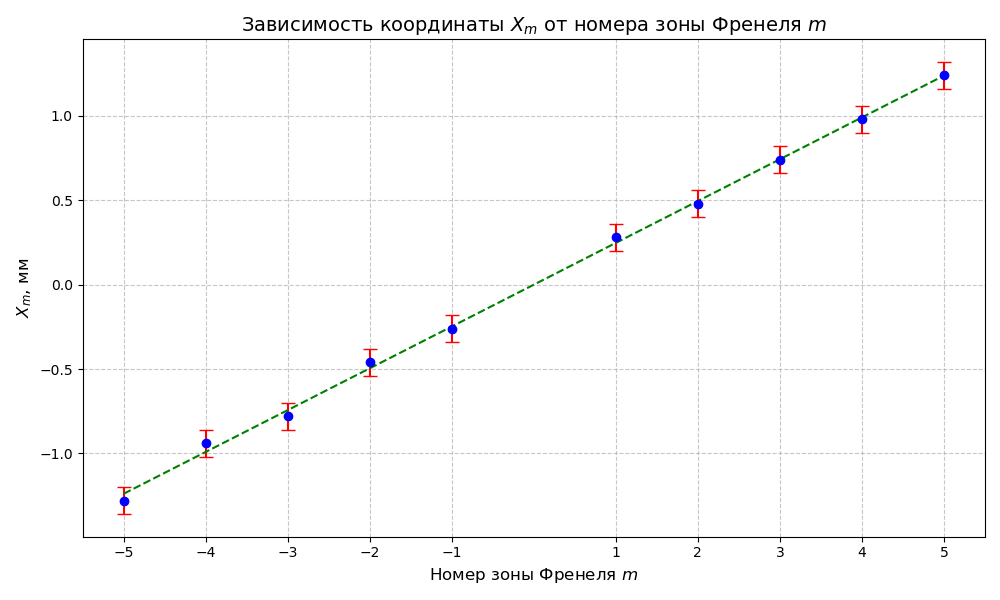
\includegraphics[width=18cm]{images/plot_B.png}
    \caption{К определению ширины щели $b$ в случае диффракции Фраунгофера на щели}\label{fig:plot_B}
\end{figure}


\subsection*{В) Дифракция Фраунгофера на двух щелях}
\indent
Два дифракционных изображения входной щели, одно из которых образовано лучами, прошедшими через левую, а другое - через правую щели, накладываются друг на друга.
Угловая координата $\theta_m$ интерференционного максимума m-го порядка определяется соотношением
\begin{equation}
    \theta_m = \frac{m\lambda}{d}
\end{equation}
где d — расстояние между щелями. Линейное расстояние $\delta x$ между соседними интерференционными полосами в плоскости П:
\begin{equation}
    \delta x = f_2\frac{\lambda}{d} \label{eq:fraunogofer2_1}
\end{equation}
Оценим число n интерференционных полос,укладывающихся в области центрального дифракционного максимума.
\newpage
\begin{figure}
    \centering
    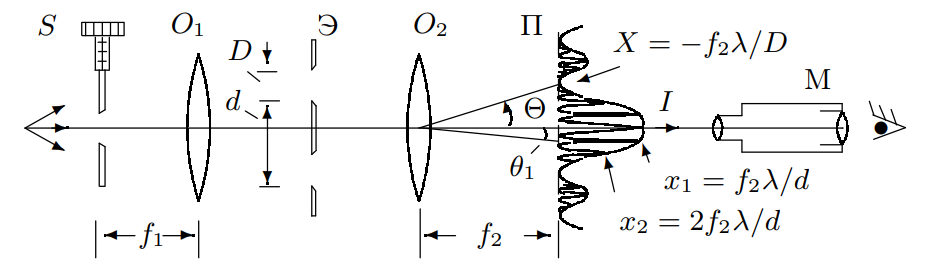
\includegraphics[width=14cm]{images/fraungofer_3.png}
    \caption{Схема установки для наблюдения дифракции Фраунгофера на двух щелях}
\end{figure}

Полная ширина главного максимума равна $2f_2\lambda / b$. Тогда число n интерференционных полос,
укладывающихся в области центрального дифракционного максимума:
\begin{equation}
    n =\frac{2\lambda f_2}{b}\frac{1}{\delta x} = \frac{2d}{b}\label{eq:fraunogofer2_2}
\end{equation}
\indent
При дифракции света на двух щелях чёткая система интерференционных полос наблюдается только при достаточно узкой ширине входной щели S, которую можно рассматривать как протяжённый источник света размером b. Для наблюдения интерференции необходимо, чтобы
расстояние d между щелями не превышало радиуса когерентности:
\begin{equation}
    d \le \frac{\lambda}{b}f_1
\end{equation}

С помощью микрометрического винта поперечных салазок микроскопа определили координаты самых удалённых друг от друга тёмных полос
внутри центрального максимума $\mathbf{l = 0.34 \pm 0.01}$ \textbf{мм} и просчитали число светлых промежутков между ними $\mathbf{n = 12}$. Измерьте ширину центрального максимума. Отсюда получаем расстояние между соседними полосами:
$$
\mathbf{\delta x = \frac{l}{n} = 28.3 \pm 0.8} \textbf{ мкм}
$$
Расстояние между щелями (\ref{eq:fraunogofer2_1} ) и ширина щели:
$$
\mathbf{d = f_2\frac{\lambda}{\delta x} = 2.31 \pm 0.07}\textbf{ мм};\text{  } 
\mathbf{b = 0.36\pm 0.01}\textbf{ мм}
$$
Найдем число полос внутри главного максимума(\ref{eq:fraunogofer2_2}):
$$
\mathbf{n = 12.9 \pm 0.6}
$$
\indent
Исследовали влияние пространственной когерентности на видность интерференционной картины. Для этого, расширяя входную щель S, подобрали такую ширину щели $\mathbf{b_0 = 27 \pm 1}$ \textbf{ мкм}, при которой наступает первое исчезновение интерференционных полос. Теоретическая величина для $\mathbf{b_0 = f_1\lambda/d = 23.3\pm0.6}$ \textbf{ мкм}.

\subsection*{Г) Влияние дифракции на разрешающую способность оптического инструмента}

\begin{figure}[h!]
    \centering
    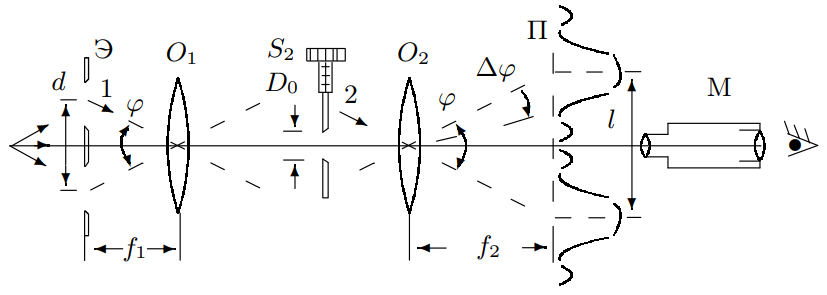
\includegraphics[width=12cm]{images/setup4.png}
    \caption{Схема установки для исследования разрешающей способности оптического инструмента}
\end{figure}
\indent
Линзы O1 и O2 в отсутствие щели S2 создают в плоскости П изображение щели S1, и это изображение рассматривается в микроскоп М. Таким образом, нашу установку можно рассматривать как оптический инструмент, предназначенный для получения
изображения предмета. При этом коллиматор (щель S1 и объектив O1)
является моделью далёкого предмета, а объектив O2 и микроскоп М
составляют зрительную трубу, наведённую на этот предмет.
Щель S2, установленная непосредственно перед объективом O2, позволяет изменять эффективный размер объектива и, следовательно, разрешающую способность оптической системы.
\indent
Поместим вместо щели S1 экран Э с двумя узкими щелями, расстояние между которыми равно $d$. Тогда расстояние $l$ между
изображениями щелей в плоскости П равно:
\begin{equation}
    l = \varphi f_2 = d\frac{f_2}{f_1}
\end{equation}
А ширина каждого изображения равна:
\begin{equation}
    \delta x \approx \frac{\lambda}{b}f_2
\end{equation}

Критерий Рэлея: изображения считаются различимыми,когда полуширина дифракционного изображения $\delta x$ совпадает с расстоянием $l$ между изображениями отдельных щелей:
\begin{equation}
    \delta x \sim l \Rightarrow \text{   } \frac{\lambda}{b} \sim \frac{d}{f_1}\label{qe:reley}
\end{equation}
\indent
Подобрали такую ширину щели $\mathbf{b_0 = 30}$ \textbf{ мкм}, чтобы изображения двух щелей почти сливались, но всё-таки ещё воспринимались раздельно.
\\\indent
Поставив двойную щель перед микроскопом, измерили с помощью
микрометрического винта поперечных салазок микроскопа расстояние $\mathbf{d = 1.7}$ \textbf{мм} между щелями. Тогда согласно критерию Рэлея \ref{qe:reley}:
$$ 
\mathbf{b_0 = f_1\frac{\lambda}{d} = 35.3\pm 0.3}\textbf{ мкм}
$$
Видим, что теоретическое и экспериментальное значение $b_0$ совпадают по порядку велечины, т.е критерий Рэлея верен.

\section*{Вывод}

\noindent
1) Сравниили полученные значения размеров зон Френеля с размером щели. Результаты получились в пределах погрешности.\\
2) Сравниили полученные значения размера щели с размером щели, измеренным микрометрическим винтом. Результаты получились в пределах погрешности. Так же проследили, как влияют изменение ширины щели и её смещение на характер дифракционной картины Фраунгофера на щели. Смещение щели S2 не приводит к смещению дифракционной картины, т.к это приводит лишь к постоянному линейному набегу фазы падающей волны, что не влияет на интенсивность (дифракционная каритна зависить от разности фаз, которая не меняется при сдвиге S2). При уменьшении ширины щели S2 дифракционная картина расширяется, что следует из формулы \ref{eq:fraunogofer}\\
3) Определили расстояние между щелями $d$ и ширину щелей $b$. Определили теоретически и экспериментально ширину щелей $b_0$, при которых наступает исчезновение интерференционных полос. Значения совпадают по порядку величины.\\
4) Сравниили измеренную ширину $b_0$ щели S2 с расчётом по формуле. Результаты совпадают по порядку величины. Т.е критерий Рэлея верен.\\


